% Chapter Template

\chapter{Background Knowledge and Related Works} % Main chapter title

\label{Chapter2} % Change X to a consecutive number; for referencing this chapter elsewhere, use \ref{ChapterX}

\lhead{Chapter 2. \emph{Background Knowledge and Related Works}} % Change X to a consecutive number; this is for the header on each page - perhaps a shortened title
%----------------------------------------------------------------------------------------
%	SECTION 1
%----------------------------------------------------------------------------------------

\section{Stokes Paramters}

In many SAR architectures, the prime objective is to maximize
the measurement potential of a space-based synthetic aperture radar in response to back-scatter from a random field whose elements have unknown orientation relative to the polarity of the radar’s illumination. Measurement potential is maximized if and only if the  data products are the four Stokes parameters of the back-scattered field (or their logical equivalent)\cite{raney2006dual}.

The output from SAR which is recorded is effectively an electromagnetic field nad can be represented  by  the ellipse swept out by its electric potential vector \textit{\textbf{E}}. Stokes proved  that  such  a  field  could  be  represented  by  four real numbers, known as the Stokes parameters $(S_1,S_2,S_3,S_4)$. The  resulting  set  of four  real  numbers,  evaluated  at  each  pixel  location  in  the multilook  image  domain,  comprises  the  fundamental  output data from a SAR \cite{raney2007hybrid}.

In  general,  the  Stokes  parameters and their derived norms provide a set of tools for quantitative image classification.
%----------------------------------------------------------------------------------------
%	SECTION 2
%----------------------------------------------------------------------------------------

\section{m-$\delta$ decomposition}

Another feature that can be derived from Stokes parameters measured in the back-scattered field is the degree of polarization \textit{\textbf{m}}.

\begin{equation}
\label{eq1}
  m = ( S_2^2 + S_3^2 + S_4^2 )^\frac{1}{2}/S_1.
\end{equation}

Another parameter of interest is the relative phase between the two linear \textit{E}-vectors of the back-scattered field.
\begin{equation}
\label{eq2}
  \delta = atan( S_4 / S_3 ) 
\end{equation}
where $-180 < \delta \leq 180$ and the + or - sign of the phase indicates the rotation direction of the polarized field\cite{raney2007hybrid}. m-$\delta$ decomposition is a widely used hybrid polarimetric decomposition technique for land-use classification \cite{chirakkal2017evaluation}.

\section{One-class SVM}
Support vector machines (SVMs) are supervised learning models that analyze data and recognize patterns, and that can be used for both classification and regression tasks. Typically, the SVM algorithm is given a set of training examples labeled as belonging to one of two classes. An SVM model is based on dividing the training sample points into separate categories by as wide a gap as possible, while penalizing training samples that fall on the wrong side of the gap. The SVM model then makes predictions by assigning points to one side of the gap or the other.

Sometimes oversampling is used to replicate the existing samples so that you can create a two-class model, but it is impossible to predict all the new patterns of fraud or system faults from limited examples. Moreover, collection of even limited examples can be expensive \cite{tax2004support}.

Therefore, in one-class SVM, the support vector model is trained on data that has only one class, which is the “normal” class. It infers the properties of normal cases and from these properties can predict which examples are unlike the normal examples \cite{scholkopf2000support}. This is useful for anomaly detection because the scarcity of training examples is what defines anomalies: that is, typically there are very few examples of the network intrusion, fraud, or other anomalous behavior.

 Unlike the Binary SVM method, which tries to find an optimal hyper plane for separating two classes, the One-class SVM classifier constructs an hyper sphere that encloses regions of data distribution \cite{guerbai2014effective}. Hence, the trained One-class SVM classifier contains the maximum of samples in the minimum sphere or enclosed sphere. When a sample is outside of the hyper sphere, it is considered as outlier.

\begin{figure}[]
\centering
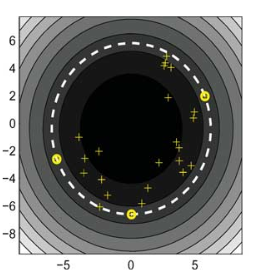
\includegraphics[width=42mm]{data5.png}
\caption{Data description trained on a banana shaped data set.}
\label{fig1}
\end{figure}

To get an intuition on how the one-class SVM works, assume we have a small 2 dimensional banana-shaped data set. we define a model which gives a closed boundary around the data: an hypersphere \cite{tax2004support}. The sphere is characterized by center \textbf{a} and radius \textbf{R} $>$ 0. We minimize the volume of the sphere by minimizing \textbf{$R^2$}, and demand that the sphere contains all training objects. In Figure \ref{fig1} support vectors are indicated by the solid circles, the dashed line is the description boundary.


%----------------------------------------------------------------------------------------
%	SECTION 3
%----------------------------------------------------------------------------------------

\section{Maximum-likelihood classifier}

The maximum likelihood classifier is one of the most popular methods of classification in remote sensing, in which a pixel with the maximum likelihood is classified into the corresponding class \cite{RSGS:2012}. Maximum Likelihood Classifier takes the variance and covariance into account.It does this by computing the distance from the pixel to each class mean value, in units of the standard deviation in that direction, and allocating the pixel to that class with the smallest value in these units of Mahalonobis distance. Mahalonobis distances vary from class to class, and indeed from direction to direction within each class.


%----------------------------------------------------------------------------------------
%	SECTION 4
%----------------------------------------------------------------------------------------

\section{Land Cover Classification using SAR}

Land cover classification is one of the most important applications in the field of polarimetric SAR research. The classification results can be either directly used in mapping and national land resource statistical research, or as the input for other applications. In the fully polarimetric SAR data, the targets’ structure information can be interpreted as the sum of surface scattering, double-bounce scattering and volume scattering. Surface scattering corresponds to rough surfaces such as bare soil and sand land. Double-bounce scattering relates to dihedral corners such as artificial targets’ ground-wall corners. Volume scattering is associated with random oriented dipoles such as the crown of a tree \cite{fang2018land}. As such, polarimetric SAR has the potential to differentiate vegetation, bare land, buildings, water bodies, and so on.

One of the most extensively used features for classification are Entropy \textbf{H},  Anisotropy \textbf{A} and scattering angle $\alpha$ \cite{lee2009polarimetric}. The complex wishart classifier described in \cite{lee2009polarimetric} takes into consideration various properties of the backscatter field. Ocean surface and flat ground typically have the characteristics of Bragg scattering (odd bounce),city
blocks, buildings, and hard targets have the characteristics of double bounce scattering (even bounce) and forest, heavy vegetation have the characteristics of volume scattering(diffuse scattering). Consequently, this classification algorithm provides information for terrain type identification. The medium’s scattering mechanisms, characterized by entropy \textit{B} and scattering angle $\alpha$, are used for classification.

%----------------------------------------------------------------------------------------
%	SECTION 5
%----------------------------------------------------------------------------------------

\section{Tools Used}

Various tools were used in order to process the SAR data, extract the features needed to classify, process the ground-truth by labelling reference pixels. All the code that was created for the project was written in python language. 
%-----------------------------------
%	SUBSECTION 1
%-----------------------------------
\subsection{PolSARpro}

PolSARpro is a project that works to provide a tool for self-education in the field of polarimetric SAR data analysis and a comprehensive suite of functions for the scientific exploitation of fully and partially polarimetric data and the development of applications for such data.

The PolSARpro software is controlled through a user-friendly, intuitive graphical interface, which enables the user to select a function, set its parameters and then run it. The software environment is flexible, developed to be accessible to a wide range of users - from novices to experts - in the field of Polarimetric SAR data processing.PolSARpro data processing routines are written in C (greater than 1000 routines) and the GUI is written in Tcl-Tk. The software is accompanied by in-depth online help, technical documentation for developers and a tutorial programme permitting self-education to a high level\cite{pottier2009overview}.

%-----------------------------------
%	SUBSECTION 2
%-----------------------------------

\subsection{QGIS}
QGIS is a popular open-source geographic information system (GIS) with advanced capabilities\cite{qgis2015qgis}. QGIS functions as GIS software, allowing users to analyze and edit spatial information, in addition to composing and exporting graphical maps. QGIS supports both raster and vector layers; vector data is stored as either point, line, or polygon features. Multiple formats of raster images are supported, and the software can geo-reference images.

\subsection{LIBSVM}
LIBSVM is an integrated software for support vector classification.It supports multi-class classification \cite{chang2011libsvm}. LIBSVM is a popular open source machine learning library, developed at the National Taiwan University and written in C++ though with a C API. LIBSVM implements the SMO algorithm for kernelized support vector machines (SVMs), supporting classification and regression.We used the python interface of LIBSVM for our One Class SVM.

%----------------------------------------------------------------------------------------
%	SECTION 2
%----------------------------------------------------------------------------------------
